\documentclass[runningheads,svgnames]{llncs}
%
\usepackage[]{graphicx}
\usepackage{amsmath}
\usepackage{hyperref}
\usepackage{cleveref}
\usepackage{booktabs}
\usepackage{orcidlink}
\usepackage{subcaption} % Addition
\usepackage{multirow} % Addition
\usepackage{tabularx} % Addition
\usepackage{siunitx} % Addition
\usepackage{scalerel}
\usepackage[inline,shortlabels]{enumitem}

% \usetikzlibrary{shadings,decorations,decorations.pathreplacing}
\renewcommand\UrlFont{\color{blue}\rmfamily}
% FIXME proper hyperref setup

\newcommand{\mcite}[1]{\text{\cite{#1}}}
\newcommand{\mref}[1]{\text{\ref{#1}}}

% Customize table rendering
\setlength{\tabcolsep}{5pt}
\renewcommand{\arraystretch}{1.4}

% Comment 
% FIXME : delete before submission :)
\newcommand{\bertrand}[1]{\textcolor{violet}{Bertrand:~#1}}
\newcommand{\nathalie}[1]{\textcolor{purple}{Nathalie:~#1}}
\newcommand{\edwin}[1]{\textcolor{pink}{Edwin:~#1}}
\newcommand{\joseph}[1]{\textcolor{red}{Joseph:~#1}}

\begin{document}
%
\title{%
Supplementary material for\\
A Benchmark of Named Entity Recognition Approaches in Historical Documents\\
Application to 19$^{th}$ Century French Directories%
}
%
\titlerunning{Supplementary material}
%
\author{%
N. Abadie\inst{1}\orcidlink{0000-0001-8741-2398} \and
E. Carlinet\inst{2}\orcidlink{0000-0001-5737-5266} \and
J. Chazalon\inst{2}\orcidlink{0000-0002-3757-074X} \and
B. Duménieu\inst{3}\orcidlink{0000-0002-2517-2058}\\
{\footnotesize \emph{all authors contributed equally}}%
}
%
\authorrunning{N. Abadie et al.}
%
\institute{%
% 1
LASTIG, Univ. Gustave Eiffel, IGN-ENSG, F-94160 Saint-Mandé, France\\
\email{nathalie-f.abadie@ign.fr}%\\
% \url{https://www.umr-lastig.fr/nathalie-abadie/}%
\and
% 2
EPITA Research \& Development Laboratory (LRDE), Le Kremlin-Bicêtre, France\\
\email{\{edwin.carlinet,joseph.chazalon\}@lrde.epita.fr}%\\
%\url{https://lrde.epita.fr}
\and
% 3
CRH-EHESS, Paris, France\\
\email{bertrand.dumenieu@ehess.fr}%\\
% \url{http://crh.ehess.fr/index.php?5206}\\
}
%
\maketitle
%
\begin{abstract}
This document contains supplementary material for the paper ``A Benchmark of Named Entity Recognition Approaches in Historical Documents ---
Application to 19$^{th}$ Century French Directories''.
\end{abstract}

% %%%%%%%%%%%%%%%%%%%%%%%%%%%%%%%%%%%%%%%%%%%%%%%%%%%%%%%%%%%%%%%%%%%%%
% #####     ##     #####    ##     ####   ######   #####
% #    #   #  #      #     #  #   #       #          #
% #    #  #    #     #    #    #   ####   #####      #
% #    #  ######     #    ######       #  #          #
% #    #  #    #     #    #    #  #    #  #          #
% #####   #    #     #    #    #   ####   ######     #
% %%%%%%%%%%%%%%%%%%%%%%%%%%%%%%%%%%%%%%%%%%%%%%%%%%%%%%%%%%%%%%%%%%%%%
\section{Dataset}

\subsection{Content}
\begin{table}[h!]
    \resizebox{\textwidth}{!}{%
    \begin{tabular}{|l|l|l|l|l|l|}
    \hline
    \multicolumn{1}{|c|}{\textbf{Directory publisher or name}} & \multicolumn{1}{c|}{\textbf{Year}} & \multicolumn{1}{c|}{\textbf{\# Col}} & \multicolumn{1}{c|}{\textbf{Index}} & \multicolumn{1}{c|}{\textbf{Entry structure}} & \multicolumn{1}{c|}{\textbf{\# Ann}}                                                                                                      
    \\ \hline
    Favre \& Duchesne & 1798 & 1 & by activity & {N [A], SN, SNUM - SEC.} & 233
    \\ \hline
    Duverneuil et La Tynna & 1801 & 1 & \begin{tabular}[c]{@{}l@{}}by activity\\ by name\end{tabular} & {N, SN, SNUM. SEC.} & \begin{tabular}[c]{@{}l@{}} 136 \\ 103\end{tabular}
    \\ \hline
    {Notables communaux de la Seine} & 1801 & 1 & by name & {N, [A,] SN[, SNUM].} & 92
    \\ \hline
    Duverneuil et La Tynna & 1805 &	2 &	\begin{tabular}[c]{@{}l@{}}by activity\\ by name\end{tabular} & \begin{tabular}[c]{@{}l@{}}N [(F)], SN, SNUM. - SEC.\\ N [(C)], [(A),] SN, SNUM. - SEC.\end{tabular} & \begin{tabular}[c]{@{}l@{}} 155 \\ 221 \end{tabular}
    \\ \hline
    Duverneuil et La Tynna & 1806 & 2 & \begin{tabular}[c]{@{}l@{}}by activity\\ by name\end{tabular} & \begin{tabular}[c]{@{}l@{}} N [(F)], SN, SNUM.\\ N [(C)], SN, SNUM.[ - SEC.]\end{tabular}. & \begin{tabular}[c]{@{}l@{}} 186\\ 0\end{tabular}
    \\ \hline
    La Tynna & 1813	& 2	& \begin{tabular}[c]{@{}l@{}}by activity\\ by name\end{tabular} & \begin{tabular}[c]{@{}l@{}} N,[A,] SN[, SNUM].\\ N, [(T)] A, SN[, SNUM] [, D].\end{tabular} & \begin{tabular}[c]{@{}l@{}} 135 \\ 177 \end{tabular}
    \\ \hline
    Panckoucke Commerces (Dulac) & 1820 & 1 & by name & N [(F)], A, [(T),] SN, SNUM[, P]. & 0
    \\ \hline
    Panckoucke Habitants (Dulac) & 1820	& 1 & by name & N [(T)], [A,] SN, SNUM [, D]. & 0
    \\ \hline
    Bottin (serie 1: 1819-1838) & 1820 & 2	& \begin{tabular}[c]{@{}l@{}}by activity\\ by name\end{tabular} & \begin{tabular}[c]{@{}l@{}} N [(F \textbar C)][T], [P], SN, SNUM.\\N [(F \textbar C)][T], A, SN, SNUM. CR\end{tabular} & \begin{tabular}[c]{@{}l@{}} 128 \\ 151 \end{tabular}
    \\ \hline
    Bottin (serie 1: 1819-1838) & 1827 & 2	& \begin{tabular}[c]{@{}l@{}}by activity\\ by name\end{tabular} & \begin{tabular}[c]{@{}l@{}}N [(F \textbar C)][T], [P], SN, SNUM.\\ N [(F \textbar C)][T], A, SN, SNUM.\end{tabular} & \begin{tabular}[c]{@{}l@{}} 228 \\ 285 \end{tabular}
    \\ \hline
    Deflandre & 1828 & 2 & \begin{tabular}[c]{@{}l@{}}by activity\\ by name\end{tabular} & \begin{tabular}[c]{@{}l@{}} N [(F \textbar C)][T], [P], SN, SNUM. \\N [(F \textbar C)][T], A, SN, SNUM.\end{tabular} & \begin{tabular}[c]{@{}l@{}}115\\ 229\end{tabular}
    \\ \hline
    Deflandre & 1829 & 2 & \begin{tabular}[c]{@{}l@{}}by activity\\ by name\end{tabular} & \begin{tabular}[c]{@{}l@{}}N [(F \textbar C)][T], [P], SN, SNUM.\\ N [(F \textbar C)][T], A, SN, SNUM.\end{tabular} & \begin{tabular}[c]{@{}l@{}}177\\ 236\end{tabular}
    \\ \hline 
    Bottin (serie 1: 1819-1838) & 1837 & 2	& \begin{tabular}[c]{@{}l@{}}by activity\\ by name\end{tabular} & \begin{tabular}[c]{@{}l@{}}N [(F \textbar C)][T], [P], SN, SNUM.\\ N [(F \textbar C)][T], [A], SN, SNUM.\end{tabular} & \begin{tabular}[c]{@{}l@{}}158\\ 557\end{tabular}
    \\ \hline
    Cambon - Almanach général & 1841 & 2 &	\begin{tabular}[c]{@{}l@{}}by activity\\ by name\end{tabular} & \begin{tabular}[c]{@{}l@{}}N [(F \textbar C)][T], [P], SN, SNUM.\\ N [(F \textbar C)][T], A, SN, SNUM.\end{tabular} & \begin{tabular}[c]{@{}l@{}}182\\ 486\end{tabular}
    \\ \hline
    Didot & 1841a &	\begin{tabular}[c]{@{}l@{}}3\\ 4\end{tabular} &	\begin{tabular}[c]{@{}l@{}}by activity \\ by name \end{tabular} & 	\begin{tabular}[c]{@{}l@{}}N [(F \textbar C)][T], [P], SN, SNUM. \\ N [(F \textbar C)][T], [A], SN, SNUM. \end{tabular} & \begin{tabular}[c]{@{}l@{}}246\\ 843\end{tabular}
    \\ \hline
    Didot & 1851a & \begin{tabular}[c]{@{}l@{}l@{}}4\\ 4\\ 5\end{tabular} & \begin{tabular}[c]{@{}l@{}l@{}}by activity\\ by name\\ by street name\end{tabular} & \begin{tabular}[c]{@{}l@{}l@{}}N [(F \textbar C)][T], [P], SN, SNUM.\\ N [(F \textbar C)][T], [A], SN, SNUM.\\SNUM N [(F \textbar C)][T], [A].\end{tabular} & \begin{tabular}[c]{@{}l@{}l@{}}309\\ 961\\ 0\end{tabular}
    \\ \hline
    Didot & 1854a & \begin{tabular}[c]{@{}l@{}l@{}}4\\ 3\\ 5\end{tabular} &	\begin{tabular}[c]{@{}l@{}l@{}} by activity \\ by name \\ by street name\end{tabular} & \begin{tabular}[c]{@{}l@{}l@{}} N [(F \textbar C)], [P], SN, SNUM [,T].\\ N [(F \textbar C)][T], [A], SN, SNUM.\\ SNUM N [(F \textbar C)][T], [A].\end{tabular} & \begin{tabular}[c]{@{}l@{}l@{}}106\\ 362\\ 0\end{tabular}
    \\ \hline
    Bottin (serie 3: 1854-1856) & 1854a & \begin{tabular}[c]{@{}l@{}l@{}}3\\ 2\\ 4\end{tabular} & \begin{tabular}[c]{@{}l@{}l@{}} by activity \\ by name \\ by street name\end{tabular} & \begin{tabular}[c]{@{}l@{}l@{}}N [(F \textbar C)], [P], SN, SNUM [,T].\\ N [(F \textbar C)][T], [A], SN, SNUM.\\ SNUM N [(F \textbar C)], [A] [,T].\end{tabular} & \begin{tabular}[c]{@{}l@{}l@{}}253\\ 633\\ 0\end{tabular}
    \\ \hline
    Didot-Bottin & 1860a	& 3	& by name & N [(F \textbar C)][T], [A], SN, SNUM. & 378
    \\ \hline
    Didot-Bottin & 1861a	& 3	& by name & N [(F \textbar C)][T], [A], SN, SNUM. & 402
    \\ \hline
    \end{tabular}%
    }
    \caption{The directories used to build our dataset. Letters next to year of publication are used to identify the volume of the directory. \# Col stands for "Number of columns", and \# Ann stands for "Number of annotated entries". Entry structure is described as follows: N - entry name (person or business); F - first name; T - honorary title; C - civility; A - activity; P - precision; SN - street name; SNUM - street number; SEC - section; D - district; CR - cross-reference; bracketed elements are optional.}
    \label{tab:directories}
    \end{table}
    
\subsubsection{Annotation tools}
To build our ground truth corpus, we annotate 78 pages randomly sampled from each of the major directory series for which we have digitised copies, using a tool developed for our project (see Figure \ref{fig:annotator}). First, the image of a given directory page is loaded. Second, entries are automatically detected and boxes are drawn around them as shown in the left panel of the Graphical User Interface (GUI). Then the text of each entry is extracted by an OCR tool and finally named entities are annotated by a NER tool: the results are displayed respectively in the first and second tabs of the right panel of the GUI. The entry detection, OCR and NER tasks are performed automatically. But as they are prone to errors, their results can be corrected manually through the GUI. In the end, the entry bounding boxes, their text, and the named entities are stored in a JSON file.

\begin{figure}[htb!]
	   \center{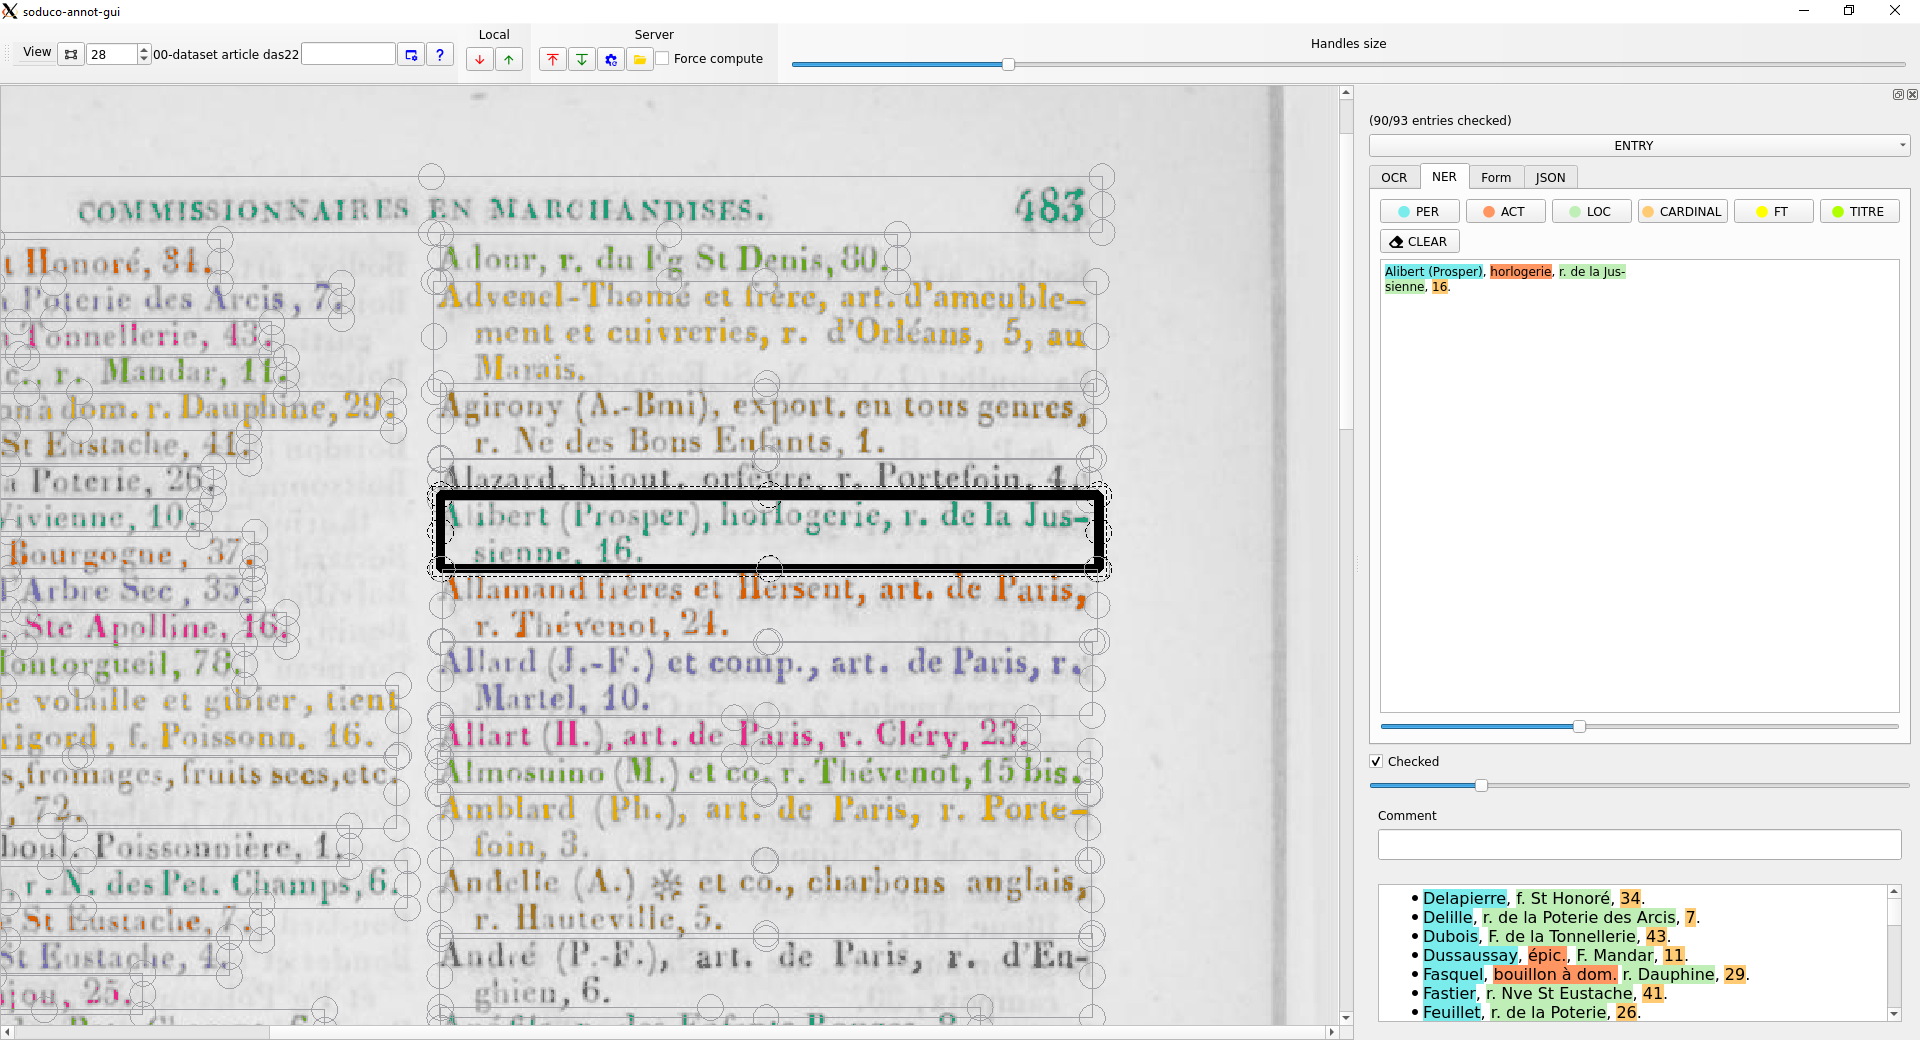
\includegraphics[width=0.9\textwidth]
	       {./images/Annot2.png}}
	  \caption{\label{fig:annotator} GUI for corpus annotation}
\end{figure}

\begin{figure}[htb!]
    \centering
    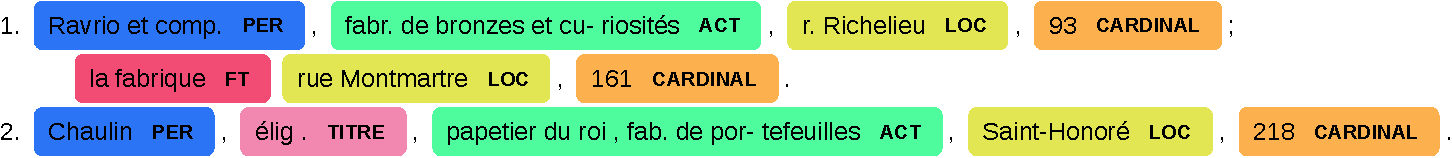
\includegraphics[width=\textwidth]{images/examples_labeled_entries.pdf}
    \caption{\label{fig:annotated-example}Two annotated entries showing the different labels used in the corpus.}
\end{figure}


\subsection{Entry segmentation}

\subsection{Line detection}
Pero OCR uses ParseNet as internal layout parser for line detection.
Pero OCR uses an LSTM engine for text line recognition.
Pero OCR generally works very well, as long as the bounding boxes of the regions to recognize are not too tightly adjusted.
Trained on newspapers in European languages by its development team.
Can output results in Latin, Greek and Cyrillic scripts, as well as some commonly-used typographic symbols.



% %%%%%%%%%%%%%%%%%%%%%%%%%%%%%%%%%%%%%%%%%%%%%%%%%%%%%%%%%%%%%%%%%%%%%
% #####   ######   ####   #    #  #        #####   ####
% #    #  #       #       #    #  #          #    #
% #    #  #####    ####   #    #  #          #     ####
% #####   #            #  #    #  #          #         #
% #   #   #       #    #  #    #  #          #    #    #
% #    #  ######   ####    ####   ######     #     ####
% %%%%%%%%%%%%%%%%%%%%%%%%%%%%%%%%%%%%%%%%%%%%%%%%%%%%%%%%%%%%%%%%%%%%%
\section{Results}



% ---- Bibliography ----
% \bibliographystyle{splncs04}
% \bibliography{ref,ref-supp}
\end{document}
